\chapter{Explainable Anomaly Detection for Communications Data: Explanation Generation Using Prior Domain Knowledge Over OneClass SVM Models} \label{chap:5-comms-xai} 

In this chapter, we focus on the first of the two real use cases within this thesis for Explainable Artificial Intelligence (XAI) for real-world applications within the telecommunications industry. Specifically for this use case, the data feeds where anomalies need to be detected and explained is communications data, such as the number of received calls in a Call Center, or the data usage (e.g. bytes) of a cell phone across a time window.

We continue the analysis carried out in \hyperref[chap:4-rule-extraction]{Chapter} \ref{chap:4-rule-extraction}, but instead of working with a general XAI proposal, we evaluate its usage within a real-world context. A real-world context, like the one we are considering, has prior domain knowledge that can be included within the explanations. Our proposal in this chapter focuses on designing an XAI method for this specific use case, including a grid search variation that finds configurations for the anomaly detection method that yield explanations aligned to the prior knowledge. 

The contributions are related to \textbf{C2.1}, introduced in \hyperref[sec:Hypotheses]{Section} \ref{sec:Hypotheses} within the \hyperref[chap:3-objetives]{Chapter} \ref{chap:3-objetives}, and appear in our granted patent \parencite{patent2019comms}.

% Vincular este capitulo con el anterior, diciendo que pasamos a estudiar XAI en un caso de uso real donde se tiene que tener en cuenta ademas info a priori. Ademas, hablar de como en ocasiones como esta sirven soluciones más sencillas que un rule extraction general.


We divide this chapter in the following three sections. \hyperref[sec:ch5-IntroComms]{Section} \ref{sec:ch5-IntroComms} presents an introduction to the use case of LUCA Comms, including a description of the product and the specific XAI needs. \hyperref[sec:ch5-GeneralProposalComms]{Section} \ref{sec:ch5-GeneralProposalComms} describes our solution, \hyperref[sec:ch5-evaluation]{Section} \ref{sec:ch5-evaluation} presents an evaluation of our proposal, and, finally, \hyperref[sec:ch5-ConclusionComms]{Section} \ref{sec:ch5-ConclusionComms} summarizes main contributions presented in this chapter.

\section{Introduction}\label{sec:ch5-IntroComms}
This first section introduces the context of LUCA Comms, and details the need of using an XAI proposal along with an anomaly detection method for both predicting and explaining outliers within communications data. \hyperref[subsec:ch5-DescriptionComms]{Subsection} \ref{subsec:ch5-DescriptionComms} presents the use case of LUCA Comms, describing the type of data considered, as well as providing a brief introduction to the product itself. \hyperref[subsec:ch5-XAI-requirements-Comms]{Subsection} \ref{subsec:ch5-XAI-requirements-Comms} focuses on the XAI aspect for anomaly detection, describing the prerequisites that the XAI proposal should include in order to be aligned with the specific business needs.


\subsection{LUCA Comms description}\label{subsec:ch5-DescriptionComms}
LUCA Comms\footnote{The brand \textit{LUCA} has undertaken several changes due to business needs. Nonetheless, we will keep mentioning it within the product names for compliance with legacy documentations and references, in order to enhance clarity.} is a B2B (business to business) product, that receives data from the Movistar network\footnote{LUCA Comms is available in other countries, not only in Spain. In those cases, the data provider is another OB (Operating Business). However, for our analysis in this thesis, we focus on data from Spain only.} (21M mobile clients that generate 1 billion events per day) related to the usage of business lines from companies that have their communications contracted with Telefónica. These data serve as input to different analytical models that seek to extract useful insights for these companies, so that they obtain additional information about the usage that they are making of the communications services they have contracted. 

Among these analytical models and additional insights, LUCA Comms includes an anomaly detection module that provides information showing when there are anomalous patterns of the network usage for that particular company. This includes two approaches. 
First, LUCA Comms works with the mobile line usage from the employees of a company. Thus, a first context is providing information about the mobile lines from the company that have an anomalous behaviour related to other similar lines from the company and for the same type of mobile traffic. For instance, a company can detect if a mobile line from the sales department is having an anomalous outbound roaming traffic compared to other lines from the same department (sales) and for the same type of traffic (outbound roaming) on a specific day of week (e.g. Mondays).
Second, Luca Comms works with the calls received by the lines of a company (e.g. inside a Call Center). Because of that, another relevant need is detecting anomalies within the received calls, showing when there is an excessive number of calls (or the opposite). For instance, the Call Center of an insurance company can see whether the number of calls received on a particular day for a specific service (e.g. lines associated to hiring products) are normal or not (they are anomalies because the volume is too high or too low for that service in that particular date).

\hyperref[fig:ch5-comms-description]{Figure} \ref{fig:ch5-comms-description} shows a high-level schema of the product, where we see how data provided by the Telefónica network is combined with client specific data (e.g. the name of the Call Center service associated to several lines) for generating the insights within the product.

\begin{figure}[h!]
\centering
  \begin{tabular}{c@{\qquad}c@{\qquad}c}
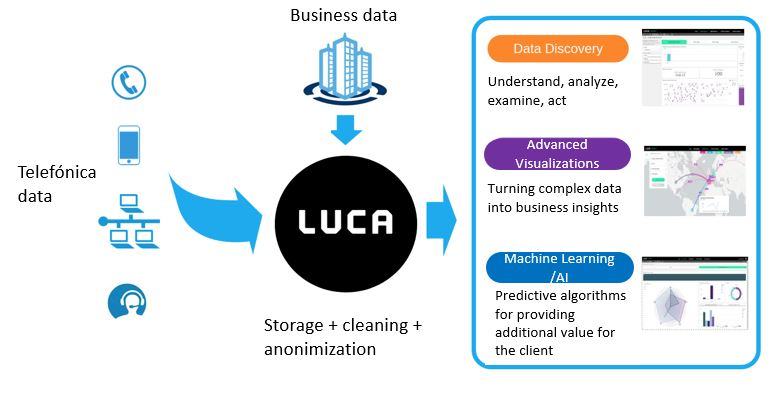
\includegraphics[width=0.90\columnwidth]{figures/chapter5_LucaComms/CommsDescription.JPG}
  \end{tabular} 
  \caption{Schema of LUCA Comms \parencite{patent2019comms}: It combines Telefónica's data with client specific data for generating the business insights within the product. \label{fig:ch5-comms-description}}
\end{figure}

Within these two anomaly detection needs, LUCA Comms is using a OneClass Support Vector Machine (OCSVM) algorithm for detecting data outliers. One of the reasons behind it is that OCSVM is an algorithm well-suited for detecting anomalies when using data sets that include temporal data \parencite{ma2003time}, as it is the case of LUCA Comms. However, deteting anomalies and providing a binary output is not enough, since customers want to know \textit{why} a specific data point is anomalous, and \textit{what} should have happened for it to be an inlier. This is why we needed to develop an Explainable AI (XAI) proposal that provides explanations that answer those questions, using as input the results from the OCSVM model.

\subsection{Specifications for explainability}\label{subsec:ch5-XAI-requirements-Comms}
As we already mentioned, LUCA Comms includes several OCSVM models, with a RBF (radial basis function) kernel, for predicting anomalies over different data sets. Nonetheless, all those data sets have in common one thing: there is only one numerical feature (e.g. bytes or number of calls), together with several categorical ones (e.g. day of week, if it is a holiday or not...). This characteristic of the data sets involved is an important detail that we will consider within our explainability approaches.
Along with this, the \textbf{business requirements} that should be met by the explanations are summarized as follows:
\begin{itemize}
    \item[\textbf{1.}] \textbf{Local explanations:} Explanations should justify why a specific data point is an anomaly.
    \item[\textbf{2.}] \textbf{Human-friendly:} Explanations should be easily understood by end-users of LUCA Comms. Thus, the features involved in the explanations must be comprehensible for them.
    \item[\textbf{3.}] \textbf{Counterfactual:} Explanations should indicate why a data point is an anomaly by indicating the changes that would turn the outlier into an inlier.
    \item[\textbf{4.}] The explanation generation method needs to be able to deal with \textbf{both numerical and categorical features}. %should show the counterfactual \textbf{changes in the numerical feature only}, within the context of specific combinations of categorical ones, However, it does not need to show counterfactual changes between categorical features.
\end{itemize}

%Without considering the underlying OCSVM ML model, those requirements could be met by a simple model such as a box-plot. Considering the subsets corresponding to each combination of categorical features, we could detect the anomalies through the box-plot whiskers. This is a whitebox model in itself, since the output shows directly in a visual way the numerical amount that should be changed in the numerical feature in order to turn an outlier into an inlier, for a specific combination of categorical features. However, there are two problems with this approach. 
%First, a box-plot will detect the anomalies for the subset of categorical combinations \textit{independently}, without considering the information of the other combinations. Thus, the anomalies in the number of received calls in a call center for a specific day of week and for a specific service will be obtained independently from the anomalies detected at that same service another day of the week, or independently from the anomalies detected in another service. 
%Second, using a box-plot approach will discard the OCSVM proposal, which was already validated for LUCA Comms. 
%With that, our goal is to obtain explanations that are \textit{similar} in structure to those of a box-plot, but by using the anomalies detected from an OCSVM model.

Without considering the underlying OCSVM ML model, those requirements could be met by a simple model such as a box-plot. Considering the subsets corresponding to each combination of categorical features, we could detect the anomalies through the box-plot whiskers. This is a whitebox model in itself, since the output shows directly in a visual way the numerical amount that should be changed in the numerical feature in order to turn an outlier into an inlier, for a specific combination of categorical features. However, there is a problem with this approach: a box-plot will detect the anomalies for the subset of categorical combinations \textit{independently}, without considering the information of the other combinations. Thus, the anomalies in the number of received calls in a call center for a specific day of week and for a specific service will be obtained independently from the anomalies detected at that same service another day of the week, or independently from the anomalies detected in another service. With that, our goal is to obtain explanations that are \textit{similar} in structure to those of a box-plot, but by using the anomalies detected from an OCSVM model.


\section{XAI proposal for explaining communications data}\label{sec:ch5-GeneralProposalComms}

In this section, we describe our proposal for predicting and explaining anomalies within communications data, within the use case of LUCA Comms.

The general process followed by LUCA Comms for detecting anomalies is detailed in \hyperref[fig:ch5-flowchart-comms]{Figure} \ref{fig:ch5-flowchart-comms}. First, using historical data, it finds the hyperparameters for the OCSVM through a grid search method that integrates prior domain knowledge in order to find hyperparameters combinations that yield results aligned with it. This step is described in \hyperref[subsec:ch5-HyperparamsComms]{Subsection} \ref{subsec:ch5-HyperparamsComms}. After that, it trains the OCSVM model with those hyperparameters, and applies our specific proposal for extracting the explanations, which includes a visual and counterfactual components. This is detailed in \hyperref[subsec:ch5-AnomalyLimitsComms]{Subsection} \ref{subsec:ch5-AnomalyLimitsComms}. Then, it both applies those limits to predict and explain the anomalies, both over the historical data used for training, as well as over new data that arrives in the system. New data can be included within the historical data when there is a need for model retraining. This is visualized through LUCA Comms application, as detailed in \hyperref[subsec:ch5-finalresult]{Subsection} \ref{subsec:ch5-finalresult}.

\begin{figure}[h!]
\centering
  \begin{tabular}{c@{\qquad}c@{\qquad}c}
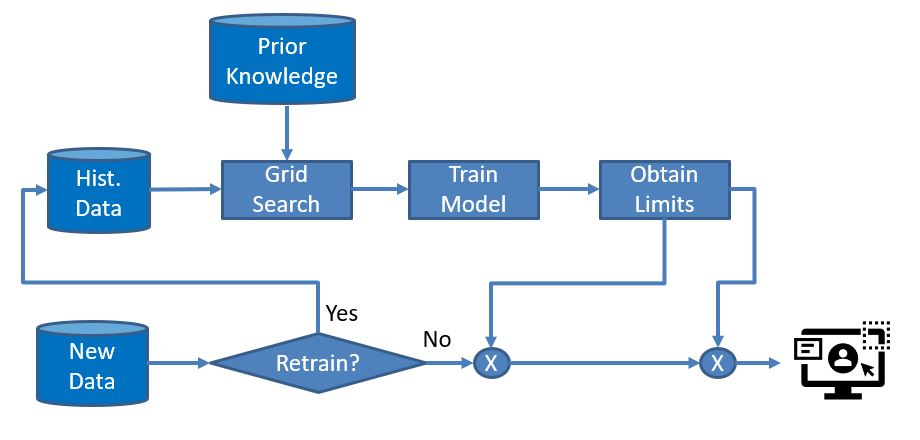
\includegraphics[width=0.80\columnwidth]{figures/chapter5_LucaComms/FlowChartComms.JPG}
  \end{tabular} 
  \caption{Flowchart describing the anomaly detection process of LUCA Comms \parencite{patent2019comms}\label{fig:ch5-flowchart-comms}}
\end{figure}


\subsection{Limit generation for visual and counterfactual explanations}\label{subsec:ch5-AnomalyLimitsComms}

In this subsection, we explain the method followed by our proposal for generating explanations over a blackbox OCSVM model for anomaly detection. As already mentioned in \hyperref[subsec:ch5-XAI-requirements-Comms]{Subsection} \ref{subsec:ch5-XAI-requirements-Comms}, the aim is to provide explanations from a OCSVM model that are visually similar to those of a box-plot, considering that there is only one numerical feature, and explaining the counterfactual changes that turn outliers into inliers within the isolated contexts of the different combinations of categorical values.

With that, the intuition behind our proposal is to first obtain the anomalies with the OCSVM, then filter the results for each combination of categorical values, and obtain the corresponding numerical value limit that differentiates inliers from outliers for each one of them, based on the information of the algorithm decision frontier. This is done by performing a \textbf{systematic random sampling} of values between the inliers and outliers for each categorical combination, and predicting their anomaly values with the ML model. Then, based on that information, we can infer the position of the decision frontier for that categorical combination. An example of the input and the output results is shown in \hyperref[fig:ch5-comms-limits-objective]{Figure} \ref{fig:ch5-comms-limits-objective}.

\begin{figure}[h!]
\centering
  \begin{tabular}{c@{\qquad}c@{\qquad}c}
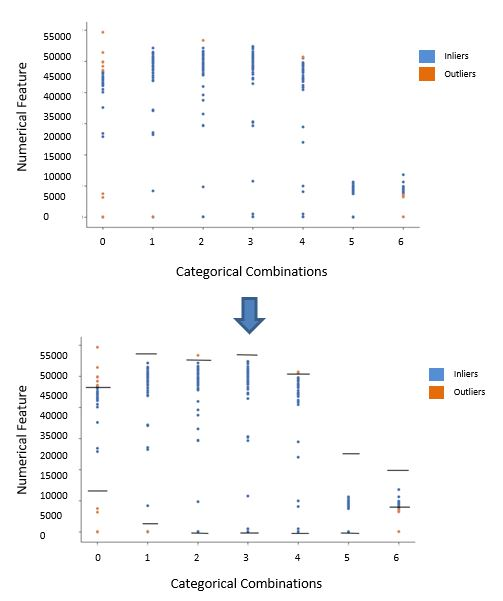
\includegraphics[width=0.70\columnwidth]{figures/chapter5_LucaComms/CommsLimits_Objective.JPG}
  \end{tabular} 
  \caption{Limit result: we aim to extract a reference value for the numerical feature and for each categorical feature combination by performing a systematic random sampling of values between them and predicting their values with the ML model. Y-axis represents the numerical variable, and X-axis a specific combination of categorical feature values \label{fig:ch5-comms-limits-objective}}
\end{figure}

The advantage of this approach is that we do not require the information of the position of the decision frontier by itself, thus providing a model-agnostic approach that could be applied over any black-box model, provided that the data set consists in one numerical feature and several categorical ones. 

The proposal for obtaining these limits for providing visual and counterfactual explanations corresponds to the contribution \textbf{TC6}, which was introduced within \hyperref[sec:Hypotheses]{Section} \ref{sec:Hypotheses}.

\hyperref[alg:ch5-ocsvm-comms-limits]{Algorithm} \ref{alg:ch5-ocsvm-comms-limits} describes in detail the process followed for generating the limits that will act as visual and counterfactual explanations over the results from the OCSVM model. It receives the input dataframe $X_i$, the numerical column name ($col\_name$), the list of categorical features ($l\_f$), the trained model, a constant for the number of random samples $N$, and coefficients for the upper/lower limits ($C_{sup}$ and $C_{inf}$ respectively). With that, it first gets the available combination of categorical columns with $unique(X_i[l_f])$. Then, it scales the data for the OCSVM model predictions and gets the anomaly predictions $X_a$. After that, it iterates through every categorical combination, and obtains the upper/lower inlier values for that subset of data. It also obtains the closest outliers to those inlier value references (the first outlier above the maximum inlier, and the first below the minimum inlier). If there are no outliers above/below within the dataset for that combination, the upper/lower reference is defined with an arbitrary offset over/under the upper/lower inliers. Then, we apply a \textbf{systematic random sampling} in order to obtain $N$ random points between the reference inlier and the reference outliers. Using those random samples, we obtain the model predictions, and we get the furthest random inliers to the upper/lower inliers. Those inliers will be the limits used for the explanations. In case all the random samples above/below are outliers, then the upper/lower inliers will be directly used as limits.

\hyperref[fig:ch5-anomaly-limit-example]{Figure} \ref{fig:ch5-anomaly-limit-example} serves as an example for the aforementioned algorithmic logic, where X-axis represents the categorical combinations and Y-axis the numerical feature. For category '0', since there are outliers above and below the inliers, the random sampling would be performed between them, in order to infer the anomaly limit (green line). For category '1', the same would be applied for the lower limit. However, since there are no outliers above the maximum inlier, the algorithm would first set an arbitrary high value and then perform the random sampling between that value and the highest outlier, yielding the limit after that. 


% Limit Generation
\begin{algorithm}[]
\caption{Limit generation for XAI over OCSVM}\label{alg:ch5-ocsvm-comms-limits}
\begin{algorithmic}[1]
\Procedure{generateLimits}{$X_{i}, col\_name, l_f, model, N, C_{sup}, C_{inf}$}

    % Get categorical combs
    \State $d_{comb} \gets unique(X_i[l_f])$
    
    % Data Preparation
    \State $X, scaler \gets scaling(X, l_f)$
    
    % Get predictions
    \State $X_{a} \gets scaler.unscale(model.predict(X, scaler))$ 
    
    % Store results
    \State $d\_limits \gets dict()$
    
    % Iter per categ. comb 
    \For{$comb \in d_{comb}$}
        % Iter params & min/max inliers
        \State $X\_iter \gets X_{a}[l_f = comb]$
        \State $X_{in} \gets X_{a}[anomalies = False]$ 
        \State $X_{out} \gets X_{a}[anomalies = True]$ 
        \State $min_{in}, max_{in} \gets MinMax(X_{in}[col\_name])$
        \State $ref\_above_{out} \gets min(X_{out}[col\_name] \geq max_{in})$
        \If{$len(ref\_above_{out}) = 0$}
            \State $ref\_above_{out} \gets C_{sup} \times max_{in}$
        \EndIf
        \State $ref\_below_{out} \gets max(X_{out}[col\_name] \leq min_{in})$
        \If{$len(ref\_below_{out}) = 0$}
            \State $ref\_below_{out} \gets C_{inf} \times min_{in}$
        \EndIf
        
        % Get random sampling
        \State $X_{above} \gets randomSample(max_{in}, ref\_above_{out}, l_f, N)$
        \State $X_{below} \gets randomSample(min_{in}, ref\_below_{out}, l_f, N)$
        \State
        % Get predictions & keep outliers only
        \State $X_{above} \gets model.predict(scaler.scale(X_{above}))$
        \State $X_{above} \gets scaler.unscale(X_{above})$
        \State $X_{above} \gets X_{above}[anomalies = False]$
        \State $X_{below} \gets model.predict(scaler.scale(X_{below}))$
        \State $X_{below} \gets scaler.unscale(X_{below})$
        \State $X_{below} \gets X_{below}[anomalies = False]$
        \State
        % Inliers above & below
        \If{$len(X_{above}) > 0$ $\&$ $len(X_{below})>0$} 
            % Keep as reference the upper random inlier
            \State $lim_{sup} \gets max(sort(X_{above}[col\_name], asc=False))$
            \State $lim_{inf} \gets min(sort(X_{below}[col\_name], asc=False))$
        
        % All points above are outliers
        \ElsIf{$len(X_{above}) > 0$ $\&$ $len(X_{below})=0$} 
            % Keep as reference directly the upper inlier
            \State $lim_{sup} \gets max_{in}$
            \State $lim_{inf} \gets min(sort(X_{below}[col\_name], asc=False))$
        
        % All points below are outliers
        \ElsIf{$len(X_{above}) = 0$ $\&$ $len(X_{below})>0$} 
            % Keep as reference directly the lower inlier
            \State $lim_{sup} \gets max(sort(X_{above}[col\_name], asc=False))$
            \State $lim_{inf} \gets min_{in}$
        
        % All anomalies
        \Else
            % Keep as reference directly the upper/lower inliers
            \State $lim_{sup} \gets max_{in}$
            \State $lim_{inf} \gets min_{in}$
        
        \EndIf
        
    \State $d\_limits[comb][lim_{sup}] \gets lim_{sup}$
    \State $d\_limits[comb][lim_{inf}] \gets lim_{inf}$
    \EndFor

\State \textbf{return} $d\_limits$

\EndProcedure
\end{algorithmic}
\end{algorithm}

\begin{figure}[h!]
\centering
  \begin{tabular}{c@{\qquad}c@{\qquad}c}
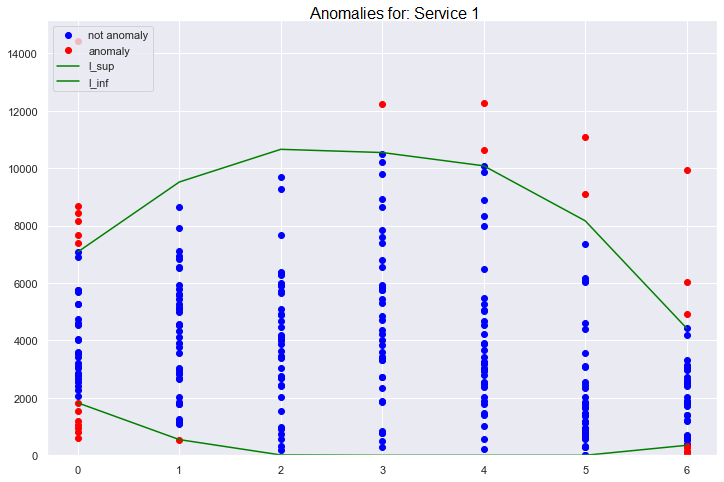
\includegraphics[width=0.70\columnwidth]{figures/chapter5_LucaComms/AnomalyLimits_example.png}
  \end{tabular} 
  \caption{An example of the anomaly limit generation, where the logic depends on whether there are anomalies above/below the inliers for each category or not. \label{fig:ch5-anomaly-limit-example}}
\end{figure}


\subsection{Hyperparameter search}\label{subsec:ch5-HyperparamsComms}

The method for obtaining the limits, described in \hyperref[subsec:ch5-AnomalyLimitsComms]{Subsection} \ref{subsec:ch5-AnomalyLimitsComms} is only suitable for when there are no outliers in the middle of the inliers. This is shown in \hyperref[fig:ch5-anomaly-limit-problem]{Figure} \ref{fig:ch5-anomaly-limit-problem}, where there are outliers between the inliers. This is something that may appear within the context we are working with, since an OSCVM that uses a RBF kernel may have more than one \textit{landmark}. When that is the case, there may be more than one upper and one lower limit that separates inliers from outliers per each categorical value combination. 

\begin{figure}[h!]
\centering
  \begin{tabular}{c@{\qquad}c@{\qquad}c}
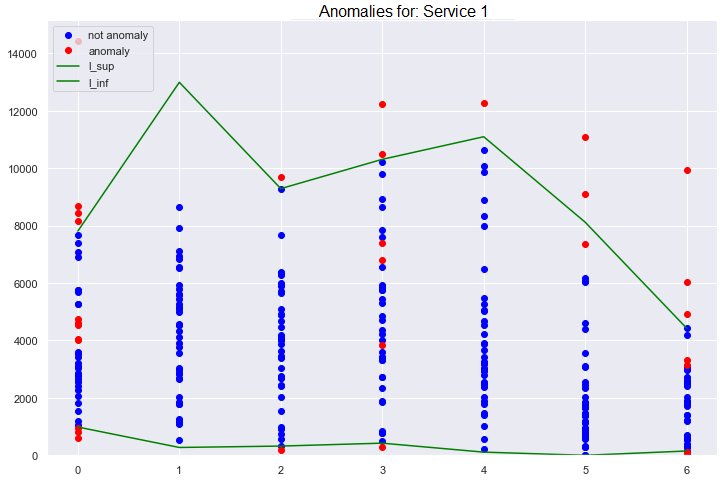
\includegraphics[width=0.70\columnwidth]{figures/chapter5_LucaComms/AnomalyLimits_example_problem.png}
  \end{tabular} 
  \caption{Inferring the limits based on the random sampling proposal already mentioned is not suitable for when there are anomalies within the inliers. \label{fig:ch5-anomaly-limit-problem}}
\end{figure}

This problem highlights an additional business need: the explanations should only show outliers above/below the inliers. It would not be helpful to indicate, for instance, that an amount of received calls in a particular call center service is \textit{not anomalous} if it is between a range of values or between another range of values, but in the middle of those ranges, the values are anomalous. This can be seen, for instance, at the categorical combination of 0 in \hyperref[fig:ch5-anomaly-limit-problem]{Figure} \ref{fig:ch5-anomaly-limit-problem}. The explanations should consider a \textbf{prior domain knowledge}: anomalies should only be above or below the inliers, but not between them. In this case, this prior domain knowledge is in fact a \textbf{rule} that should be taken into account during the explanation generation process. 

Following the taxonomy of \parencite{beckh2021explainable}, which covers different approaches for integrating prior knowledge in the explanation generation, we need an approach within the context of \textbf{Informed Machine Learning}\footnote{It is important to note that the article \parencite{beckh2021explainable} was developed after our proposal. Thus, we did not have this taxonomy at the beginning for guiding our research. Nonetheless, our proposal falls inside the aforementioned category.}. This is because we are not using a post-hoc model for building the explanations. Instead, we are obtaining them directly from the information of the model (the decision frontier). Thus, the prior knowledge needs to be included at the ML model level. 
Our proposal to include this knowledge is placed within the \textbf{hypothesis set} type of knowledge integration. In particular, we aim to include that knowledge within the hyperparameter grid search, in order to choose the best parameter configuration that is also aligned with that business rule.

OCSVM has two important hyperparameters to optimize:
\begin{itemize}
    \item $\gamma$: It is the \textit{rejection rate}, which defines the maximum limit for the fraction of points that could be considered an anomaly.
    \item $\nu$: It is the fraction for the limit of the number of support vectors. This limits the number of support vectors used, defining the minimum limit for the fraction of points that could be used as support vectors.
\end{itemize}

Those parameters lead to the following trade off \parencite{xiao2014parameter}:
\begin{itemize}
    \item \textit{Decrease the rejection rate}: \textit{increases} the space for non-anomalous points; fewer anomalies detected. This may lead to overfitting.
    \item \textit{Increase the rejection rate}: \textit{decreases} the space for non-anomalous points; more anomalies detected. this may lead to underfitting.
\end{itemize}
Even though the previous points define the trade off for $\gamma$, the problem is similar with $\nu$.

However, OCSVM is used as an unsupervised ML algorithm, which means that the hyperparameter optimization, and its combination with prior domain knowledge, should also be done in an unsupervised manner.

The MIES (\textit{measure the distance from samples to enclosing surfaces}) algorithm \parencite{xiao2014parameter} proposes an approach for computing a score that can be used for finding the best hyperparameter configuration. It proposes a way to perform a grid search for OCSVM as long as the kernel used is RBF (which is the one that we are already using within our approach). The method calculates the normalized distance (ND) of the data (target data) to the decision frontier, for both data points outside the decision boundary (edge patterns, EP), and within it (interior patterns, IP), and with that information it decides which combination of hyperparameters is optimal.
To do that, it first calculates the ND for the IPs. The IPs should be as far away as possible from the decision frontier. This will avoid underfitting (too many anomalies detected), since the obtained decision frontier will not be too close to the inliers. Because of this, the optimal choice would be the one that maximizes this criterion. But that criterion alone is not enough because it will lead to overfitting due to the large non-anomalous space that would be generated (and fewer anomalies would be detected). Therefore, another criterion to consider is the ND for EP. They should be as close as possible to the decision frontier. That way, that decision frontier would respect and better capture the distribution of the underlying data. This is summarized in \hyperref[fig:ch5-mies-example]{Figure} \ref{fig:ch5-mies-example}.

\begin{figure}[h!]
\centering
  \begin{tabular}{c@{\qquad}c@{\qquad}c}
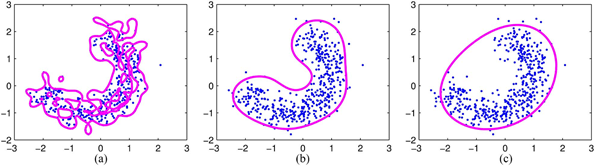
\includegraphics[width=0.90\columnwidth]{figures/chapter5_LucaComms/MIES_examples.png}
  \end{tabular} 
  \caption{Some examples of decision frontiers obtained for different use cases \parencite{xiao2014parameter}. Example (c) shows a decision frontier obtained by trying only to maximize the distance from the interior points (IPs) to the decision frontier. Example (a) shows a decision frontier obtained only by trying to minimize the distance from the edge points (EPs) to the decision frontier. The optimal situation is (b) where both factors are taken into account. \label{fig:ch5-mies-example}}
\end{figure}

With that, the objective function from MIES is the following one:
$fo(s) = max ND(x_i) - max ND(x_j)$
With $x_i$ the IP, $x_j$ the EP, and ND the normalized distance. The $max$ function returns the maximum distance value among all the data points for each of those two groups, IP and EP. 
The normalized distance is obtained as follows:
$ND = frac{d}{1 - d_{\pi}}$ 
With $d$ the distance of each data point to the decision frontier, and $d_{\pi}$ a reference distance computed between the origin of coordinates (OO) and an hyperplane obtained from the decision frontier.

Using that hyperparameter selection as a reference, we propose an algorithm that first filters out hyperparameter configuration that do not comply with the prior domain knowledge, and then applies MIES algorithm in order to find the best one of them. \hyperref[alg:ch5-ocsvm-comms-gridsearch]{Algorithm} \ref{alg:ch5-ocsvm-comms-gridsearch} describes the process followed. It receives the input dataframe $X_i$, the numerical column name ($col\_name$), the list of categorical features ($l\_f$), and a dictionary $dct_{hyper}$ with the different hyperparameter ranges for $\nu$ and $\gamma$. With that, it first gets the available combination of categorical columns with $unique(X_i[l_f])$. Then, it scales the data for the OCSVM model training and the MIES score. After that, it initializes a dictionary with the results (hyperparameter values and metric scoring) $d\_ref$. Following this, it iterates through the different hyperparameters, and gets the corresponding model predictions with $fitPredict(X, scaler)$. The values in $X_a$ are unscaled. Before computing the MIES metric, the algorithms checks that no outliers are between the inliers for each categorical combination. If at least one categorical combination has outliers between the inliers, that hyperparameter configuration is skipped. When there are no outliers between the inliers, the algorithm proceeds to obtain the MIES metric score ($MIES(X, scaler, l_s)$), and when that score improves the score from the previous iteration, it keeps it as the best reference. 
The algorithm finally returns the MIES score, along with the corresponding $\nu$ and $\gamma$ for that best hyperparameter configuration.

% MIES Variation
\begin{algorithm}[]
\caption{Grid search with prior knowledge along with MIES}\label{alg:ch5-ocsvm-comms-gridsearch}
\begin{algorithmic}[1]
\Procedure{gridSearch}{$X_{i}, col\_name, l_f, dct_{hyper}$}

    % Get categorical combs
    \State $d_{comb} \gets unique(X_i[l_f])$
    
    % Data Preparation
    \State $X, scaler \gets scaling(X, l_f)$
    
    % Default reference
    \State $d\_ref \gets dict()$
    \State $d\_ref[score] \gets -\infty$
    \State $d\_ref[\nu] \gets null$
    \State $d\_ref[\gamma] \gets null$
    
    % Iter per hyperparameter combinations
    \For{$params \in dct_{hyper}$}
    
        % Init params
        \State $d\_iter \gets dict()$
        \State $d\_iter[\nu, \gamma] \gets params[\nu, \gamma]$
        \State $flagInside \gets False$
        
        % Get predictions
        \State $X_{a} \gets scaler.unscale(fitPredict(X, scaler))$ 
        
        % Iter per categ. comb and check middle points
        \For{$comb \in d_{comb}$}
            \State $X\_iter \gets X_{a}[l_f = comb]$
            \State $min_L, max_L \gets MinMax(X\_iter[anomalies = 0][col\_name])$
            \State $X_{check} \gets X\_iter[anomalies = 1$ \& $col\_name \geq min_L$ \& $col\_name \leq max_L]$
            \If{$len(X_{check})$} 
                \State $flagInside \gets True$
            \EndIf
        \EndFor
        
        \If{$flagInside = True$}
            \State $continue$
        \EndIf
        
        % Get MIES metric if there are no middle points
        \State $dct\_results \gets MIES(X, scaler, l_s)$
        
        % Keep result as reference if better than previous
        \If{$dct\_results[score] \geq d\_ref[score]$}
            \State $d\_ref[score] \gets dct\_results[score]$
            \State $d\_ref[\nu] \gets dct\_results[\nu]$
            \State $d\_ref[\gamma] \gets dct\_results[\gamma]$
        \EndIf
        
    \EndFor
        
    \State \textbf{return} $d\_ref$
    
\EndProcedure
\end{algorithmic}
\end{algorithm}


\hyperref[alg:ch5-ocsvm-comms-gridsearch]{Algorithm} \ref{alg:ch5-ocsvm-comms-gridsearch} corresponds to the contribution \textbf{TC7}, which was introduced within \hyperref[sec:Hypotheses]{Section} \ref{sec:Hypotheses}.

\pagebreak

\subsection{Final result}\label{subsec:ch5-finalresult}


% Hablar de como se aplican las franjas que se calculan por comb de categoricas sobre cada dia luego para ver si hay o no anomalías (es decir, explicar cual es la visualizacion final, y luego vincularlo con el ejemplo del dashboard final donde se filtra por servicios)

After having the upper and lower limits of each numerical variable with respect to the different combinations of categorical ones, those limits are used for both explaining the already detected anomalies within the historical data, as well as for predicting new anomalies, as shown in \hyperref[fig:ch5-comms-anomalies-viz]{Figure} \ref{fig:ch5-comms-anomalies-viz}. There, we see how the visualization shows one plot per categorical combination for all categorical variables that are not daily-related, and then, since the X-axis includes the different dates, the limits on that day will correspond to the categorical combinations of the daily-related for that specific date (week day in our case, but there can be others, like if it is a holiday or not).

\begin{figure}[h!]
\centering
  \begin{tabular}{c@{\qquad}c@{\qquad}c}
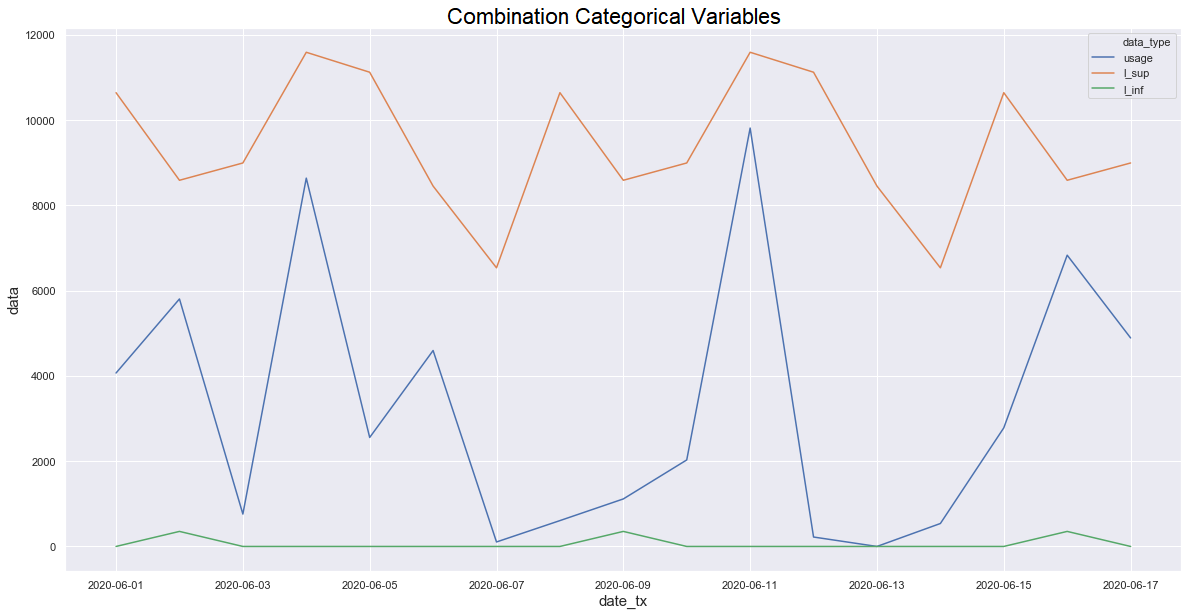
\includegraphics[width=0.9\columnwidth]{figures/chapter5_LucaComms/ThresholdsResults.png}
  \end{tabular} 
  \caption{Example of the applications of the limits over the historical data evolution \label{fig:ch5-comms-anomalies-viz}}
\end{figure}

The final visualization within LUCA Comms is shown in \hyperref[fig:ch5-comms-anomalies-result]{Figure} \ref{fig:ch5-comms-anomalies-result}. Users first select a filter for the categorical variables on the left (in our case, service name for CC or combination of organizational levels for M), the numerical variable, and then they see the data evolution for a specific period of time, with the corresponding limits, and highlighting the dates that are anomalous. Hovering over that date, they can see the counterfactual explanation, showing the actual value and the value that it should be for that date in order to be an inlier.

\begin{figure}[h!]
\centering
  \begin{tabular}{c@{\qquad}c@{\qquad}c}
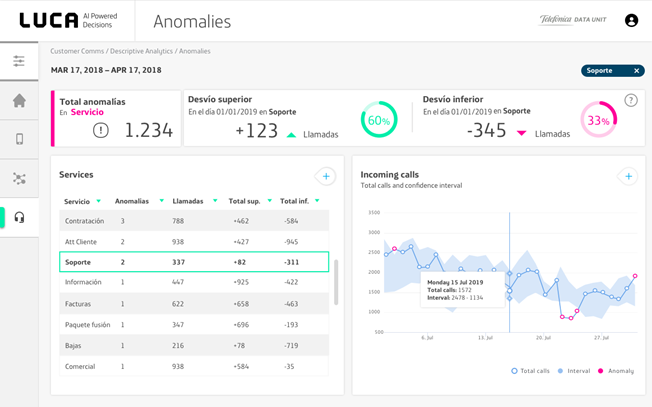
\includegraphics[width=0.9\columnwidth]{figures/chapter5_LucaComms/CommsAnomalies.png}
  \end{tabular} 
  \caption{Example of the XAI approach for anomaly detection within LUCA Comms product. \label{fig:ch5-comms-anomalies-result}}
\end{figure}

\section{Evaluation}\label{sec:ch5-evaluation}
In this section, we highlight some aspects regarding the evaluations carried out. First, we describe the datasets that we have used in \hyperref[subsec:ch5-DataComms]{Subsection} \ref{subsec:ch5-DataComms}, and then we focus on the evaluations themselves along with the hypothesis checked, in \hyperref[subsec:ch5-ResultsComms]{Subsection} \ref{subsec:ch5-ResultsComms}.

Our aim is to use this analysis for evaluating \textbf{H2}, described in \hyperref[chap:3-objetives]{Chapter} \ref{chap:3-objetives} at
\hyperref[sec:Hypotheses]{Section} \ref{sec:Hypotheses}, within the context of communications data. The reason behind it is that here, we are considering prior domain knowledge along with XAI for anomaly detection, including it for adjusting the explanations generated. Thus, we aim to check how this can indeed be done using real-world data, as well as showing how this is compatible with not having a significant decrease in the predictive power of the anomaly detection algorithm.

\subsection{Data involved}\label{subsec:ch5-DataComms}
In this subsection, we describe the data sets used for the initial validations of our proposal. We use two types of data sets, one for the usage of customer's mobile lines (M), and other regarding the received calls in lines associated to customer's services (e.g. Call Center lines, CC). The two types of data sets have in common that there is only one numerical variable, together with several categorical ones.

% Variables M y qué representan, qué variables se usan para anomalías y cómo se preprocesan
Regarding the data set for M, there are five different numerical variables that will be considered along with the categorical ones. Since we are dealing with an univariate approach regarding the numerical variable, we work with five different data sets, explaining the anomalies in each one of those variables independently, within the context of the categorical ones. Below, we indicate the different numerical variables used:

\begin{itemize}
    \item \textbf{National voice}: Minutes of voice for national calls.
    \item \textbf{Roaming out voice}: Minutes of voice for roaming out calls.
    \item \textbf{National data}: Bytes used in data traffic for national web navigation.
    \item \textbf{International voice}: Minutes of voice for international calls
    \item \textbf{Roaming data}: Bytes used in data traffic for roaming data.
\end{itemize}

For M, the categorical variables that are included as a context for the initial validations are:

\begin{itemize}
    \item \textbf{Weekday}: Day of the week associated to the traffic type.
    \item \textbf{Organizational level 2}: A organization which encloses several mobiles lines (e.g. \textit{People Analytics} department)
    \item \textbf{Organizational level 1}: A hierarchical organizational level from a company, that references the parental organization from \textbf{Organizational level 2} (e.g. \textit{Human Resources} to \textit{People Analytics} department)
\end{itemize}

% Distribucion datos M
\hyperref[table:ch5-mf-distribution]{Table} \ref{table:ch5-mf-distribution} describes the different data sets used for the validations with M, using the information of three clients. 

\begin{table}[h!]
\centering
\resizebox{0.8\textwidth}{!}{%
\begin{tabular}{@{}lllllll@{}}
\toprule
\textbf{Client} & \textbf{N Size} & \textbf{Min Date} & \textbf{Max Date} & \textbf{N Lines} & \textbf{N Org Level 1} & \textbf{N Org Level 2} \\ \midrule
C1  & 1120766 & 2019-11-08 & 2020-06-17 & 7808  & 30 & 32 \\
C2  & 3031749 & 2020-03-09 & 2020-08-31 & 20936 & 1  & 1  \\
C3      & 145398  & 2019-08-17 & 2020-06-17 & 995   & 6  & 19 \\ \bottomrule
\end{tabular}%
}
\caption{Data distribution for M, which includes the data set size, the period range considered, and the different organizational levels. C2 organizational information was not available; thus, there is a generic organization that encloses all the lines.}
\label{table:ch5-mf-distribution}
\end{table}

% Variables CC y qué representan, qué variables se usan para anomalías y cómo se preprocesan
For CC, there is only one numerical feature (number of calls), along with the categorical ones. They are described below:
\begin{itemize}
    \item \textbf{Number of calls}: Total number of calls received in a particular day for a specific service. It sums all the calls received by the lines associated to that service.
    \item \textbf{Weekday}: Day of the week associated to the daily received calls.
    \item \textbf{Service}: Service associated to several specific lines (e.g. 'Customer Support' service)
\end{itemize}

% Distribucion datos CC
\hyperref[table:ch5-cc-distribution]{Table} \ref{table:ch5-cc-distribution} describes the different data sets used for the validations with CC, using the information of three clients. 
\begin{table}[h!]
\centering
\resizebox{0.6\textwidth}{!}{%
\begin{tabular}{@{}llllll@{}}
\toprule
\textbf{Client} & \textbf{N Size} & \textbf{Min Date} & \textbf{Max Date} & \textbf{N Lines} & \textbf{N Services} \\ \midrule
C1  & 4632   & 2019-11-16 & 2020-06-17 & 52   & 47   \\
C4       & 12222  & 2019-07-04 & 2020-06-17 & 47   & 19   \\
C2 & 214590 & 2020-03-09 & 2020-08-31 & 1727 & 1727 \\ \bottomrule
\end{tabular}%
}
\caption{Data distribution for CC, which includes the data set size, the period range considered, and the different services.}
\label{table:ch5-cc-distribution}
\end{table}

Finally, in \hyperref[table:ch5-ground-truth]{Table} \ref{table:ch5-ground-truth} we see the ground truth available per client, data set and numerical variable, which includes the total data points within it along with the total daily anomalies\footnote{
Not all the data sets from \hyperref[table:ch5-cc-distribution]{Table} \ref{table:ch5-cc-distribution} or \hyperref[table:ch5-mf-distribution]{Table} \ref{table:ch5-mf-distribution} appear within this table (e.g. C2). This means that those data sets have been used for other validations (such as ensuring that there are no outliers within the inliers, or additional qualitative analyses), but not for this specific hypothesis contrast since there is not a ground truth available.}.

\begin{table}[h!]
\centering
\resizebox{0.6\textwidth}{!}{%
\begin{tabular}{@{}lllll@{}}
\toprule
\textbf{Client} & \textbf{Data set} & \textbf{Numerical variable} & \textbf{N points} & \textbf{N anomalies} \\ \midrule
C1 & CC & num\_calls           & 1362 & 171 \\
C1 & M  & international\_voice & 264  & 2   \\
C1 & M  & national\_data       & 740  & 91  \\
C1 & M  & national\_voice      & 621  & 0   \\
C1 & M  & roaming\_data        & 168  & 11  \\
C4 & CC & num\_calls           & 3078 & 548 \\
C3 & M  & international\_voice & 424  & 5   \\
C3 & M  & national\_data       & 1908 & 264 \\
C3 & M  & national\_voice      & 1480 & 58  \\
C3 & M  & roaming\_data        & 820  & 16  \\
C3 & M  & roaming\_out\_voice  & 164  & 0   \\ \bottomrule
\end{tabular}%
}
\caption{Ground truth available for the evaluations carried out.}
\label{table:ch5-ground-truth}
\end{table}

\subsection{Results}\label{subsec:ch5-ResultsComms}
As an evaluation of our proposal, we compare the results over the ground truth by two methods. First, the original MIES algorithm for finding the hyperparameters for the OCSVM models, training one model over each register in \hyperref[table:ch5-ground-truth]{Table} \ref{table:ch5-ground-truth}. Second, our proposal that combines MIES with apriori knowledge, not considering combinations that yield results that do not follow the business rule. 
For the evaluation, we carry out a Wilcoxon signed-rank test \parencite{conover1998practical} that compares the results over all the data sets by the two methods. Our hypothesis is that using our variation proposal of MIES would not significantly worsen the results over using the original MIES. This means that we can combine prior knowledge and a grid search technique in order to find reliable results that also comply with the business knowledge.
Since the hyperparameter configurations from MIES can potentially lead to more anomalies (since, besides detecting anomalies over or under the inliers, there can also be anomalies between them), we will compare the results from the False Negatives (FN) and True Positives (TP), normalizing the results with respect to the number of real anomalies for that dataset (leading to a result between 0 and 1).
Results appear in \hyperref[table:ch5-H-contrast-comms]{Table} \ref{table:ch5-H-contrast-comms}, with \textit{Reference} corresponding to the original MIES method, and \textit{New Method} to our proposal. We see how, even though the results are predictably worse for our proposal (since we are applying a constraint that may discard theoretically better configurations), they are not significantly different (using a p-value of 0.05). Thus, applying the business knowledge constraints does not significantly penalize the results obtained.

\begin{table}[h!]
\centering
\resizebox{0.6\textwidth}{!}{%
\begin{tabular}{@{}llll@{}}
\toprule
\textbf{Metric} & \textbf{Mean (Reference)} & \textbf{Mean (New Method)} & \textbf{P-value} \\ \midrule
per\_TP         & 0.61                        & 0.60                         & 0.2586           \\
per\_FN         & 0.39                        & 0.41                         & 0.2513           \\ \bottomrule
\end{tabular}%
}
\caption{Hypothesis contrast comparing TP and FN among the different grid search methods}
\label{table:ch5-H-contrast-comms}
\end{table}

With that, we validate \textbf{H2} within the context of communications data, since there are no significant changes in either of the metrics.


\section{Conclusion}\label{sec:ch5-ConclusionComms}
In this chapter, we have described our XAI proposal for explaining the anomalies detected from a OCSVM model, through visual and counterfactual explanations, within the real-world context of communications data. Our proposal generates visual explanations for a numerical feature with respect to every combination of categorical feature values using the information from the decision frontier of the ML algorithm. Along with this, we propose the usage of a grid search algorithm based on MIES that includes prior domain knowledge, so the explanations generated are aligned with it.
We carried out an empirical evaluation, where we analysed if the predictive power of OCSVM is significantly lower when we apply a constraint over the possible hyperparameter configurations for choosing only those aligned with prior domain knowledge. We saw how, even if there is a decrease in several metrics, it is not statistically significant. Thus, we can have an algorithm that provides explanations aligned with prior domain knowledge that also performs similarly to one that is free of constraints and provides explanations that may contradict that knowledge.

With that, this chapter serves for checking \textbf{H2}, described in \hyperref[sec:Hypotheses]{Section} \ref{sec:Hypotheses}, by showing how prior domain knowledge can be integrated within the XAI explanations, and this does not harm the predictive power of the model beneath them.

